\section{Великие планы}

\begin{frame}{Общие слова, план}
  \begin{itemize}
  \item Сделать абстрактную VCS.
  \item Понять, что вообще можно хранить в такой VCS.
  \end{itemize}
\end{frame}

%\begin{frame}{Ололо картинки}
%    \begin{tikzpicture}
%        [parent anchor=east,child anchor=west,grow=east,
%            sibling distance=15mm, level distance=15mm,
%            every node/.style={ball color=red,circle,text=white},
%        edge from parent/.style={draw,dashed,thick,red}]
%        \node {root}
%        child {node {left}}
%        child {node {right}
%            child {node {child}}
%            child {node {child}}
%        };
%    \end{tikzpicture}
%\end{frame}
%
\begin{frame}{ФФФФ}
    ололо
    \begin{figure}
        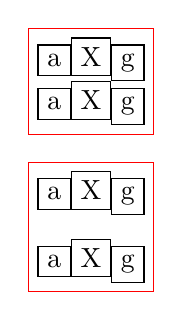
\begin{tikzpicture}
            [every node/.style={draw=black,anchor=base}]
            \matrix [draw=red]
            {
                \node {a}; & \node {X}; & \node {g}; \\
                \node {a}; & \node {X}; & \node {g}; \\
            };
            \matrix [row sep=3mm,draw=red] at (0,-2)
            {
                \node {a}; & \node {X}; & \node {g}; \\
                \node {a}; & \node {X}; & \node {g}; \\
            };
        \end{tikzpicture}
    \end{figure}
\end{frame}
